\chapter{Dataset selection}
\section{Selecting a dataset depending on the project type}
	The dataset is the fundament of a data-science project. The quality, size and closeness to reality decide the degree to which the findings can be helpful for solving real problems. 
	In this section, a classification for data-science projects is introduced.
	
	\subsection{Project Types}
\begin{table}[ht]
	\caption{Fundamental Data Science Project Types}
	\begin{tabular}{l|ll}
		\toprule
		& \textbf{Problem-First}                                                                                                              & \textbf{Data-First}                                                                                                                                                \\
		\midrule
		\vspace{0.5cm}
		Systematics                                                             & Applied Data Science                                                                                                                & Exploratory Data Science                                                                                                                                           \\
		\vspace{0.5cm}
		\begin{tabular}[c]{@{}l@{}}Underlying\\ Question\end{tabular}           & \begin{tabular}[c]{@{}l@{}}How can a problem be \\ solved?\end{tabular}                                                             & \begin{tabular}[c]{@{}l@{}}Which problems can be \\ solved with the solution?\end{tabular}                                                                         \\
		\vspace{0.5cm}
		\begin{tabular}[c]{@{}l@{}}Role of the \\ dataset\end{tabular}          & \begin{tabular}[c]{@{}l@{}}Different datasets can be \\ considered for one \\ problem statement.\end{tabular}                       & \begin{tabular}[c]{@{}l@{}}The dataset is the core of \\ the project, with a new \\ dataset, a new project begins.\end{tabular}                                    \\
		\vspace{0.5cm}
		\begin{tabular}[c]{@{}l@{}}Requirements \\ for the dataset\end{tabular} & \begin{tabular}[c]{@{}l@{}}Require a ground truth or \\ established methods for \\ evaluating the goal \\ achievement.\end{tabular} & \begin{tabular}[c]{@{}l@{}}Compared to problem-first projects, \\ larger datasets are required because\\ there is no prior assumption of \\ patterns.\end{tabular} \\
		\vspace{0.5cm}
		Fixed component                                                         & Problem statement.                                                                                                                  & Dataset.                                                                                                                                                           \\
		\vspace{0.5cm}
		Innovative Aspect                                                       & \begin{tabular}[c]{@{}l@{}}Defined during formu-\\ lation of the goal.\end{tabular}                                                 & Found during the project.                                                                                                                                         
	\end{tabular}
\end{table}

	The problem-first project type is characterized by a predefined problem statement or research goal. The underlying question is, how a specific or a set of problems can be solved \cite{dataScienceProjectTypes}.  For the selection of the dataset, this requires that goal achievement can be measured with existing ground truth. In some cases, also other methods such as expert judgements can be sufficient. In a problem-first project, different datasets can and should be considered. \cite{dataScienceProjectTypes} give the metaphor of "mining for valuable minerals or metals at a given geo- graphic location where the existence of the minerals or metals has been established".
	
	The complementary project type is the data-first project. This type is characterized by a more explorative approach, and the goal to find problems and patterns. Here, the dataset is at the core of the project and the fixed aspect of a project. In turn, this means swapping the dataset is the start of a new project. When turning to the metaphor of mining for minerals, this type of project would be the exploration of different test pits that promise mineral occurences \cite{dataScienceProjectTypes}.
	
	\subsection{Systematization of this project}
	Usually, the project type is not decided on, but implicitly arises out of environmental parameters. This is also the case in this project. While there was no initial business goal defined, a dataset was chosen and agreed upon. The decision process is detailed in the next section, \ref{data-source}. The dataset being the anchor of the project, this data science project can easily be classified as a Data-First project.
	
	\subsection{Resulting Requirements for selecting a dataset}
	In a data-first project, there is no assumption of patterns. This for once means that a large dataset is required to cover enough ground for accurate derivation of insights. Second, a data-first project does not require structured data \cite{srivastavaDataMining}. Instead, unstructured and semi-structured data is also applicable for data-first projects.
	
	
	\section{Selecting an appropriate data source}
	\label{data-source}
	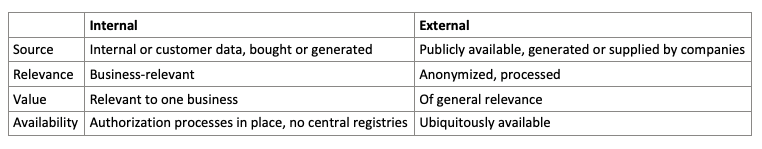
\includegraphics[height=3cm]{Bilder/internal_external.png}
	
	With the project type as a decisive factor for the dataset explained, the other evaluation criteria for the dataset is described. In the corporate environment two fundamental sources for data exist. 
	
	Firstly, data can be sourced from inside the company. This can include customer data or data generated from observation and monitoring processes inside the company. Data is either directly or very closely related to the company's business. Depending on the solution, it can be of use to customers or it can be utilized inside the company. Internally sourced data is almost exclusively rated confidential, limiting even intra-company access to it. Authorization processes and more than often not existing registries for data may hinder project progress.
	
	Secondly, data can be sourced outside the company. A vast number of online registries for data exist, both with paid and free of charge service offerings. Data sources include real-life data and data generated for educational purposes. Because of its publication, the data is stripped from all parts which could expose confidential information such as corporate secrets. Additionally, data is anonymized and processed to limit the usefulness to potential competitors.
	
	It can be stated, that both sources are suited for different goals and different contexts. For data scientists with internal sources available, this type of source seems more appealing. The resulting data sets often are of higher quality and relevance. Of course, external data sets are important especially for independent data scientists without access to paid databases.